\documentclass{../notatki}
\usepackage{physics}

\title{Wstęp do Fizyki Kwantowej}

\begin{document}

\section{Wstęp}

Przydatne wzory w jednym miejscu:
\begin{itemize}
  \item Pęd ciałą o masie $m$ i prędkości $v$:
    $$
    p = mv
    $$
  \item Energia ciała o masie $m$ i pędzie $p$: $$
    E^2 =c^2p^2 + m^2c^4
    $$
  \item Stała plancka i jej \textbf{evil twin} $$
    h = 2 \pi \hbar
    $$
  \item Prędkość fali $$
    v = \lambda \nu
    $$
\end{itemize}

\subsection{Algebra}

\textit{Z jakiegoś powodu dużą częścią zajęć była algebra, bo fizycy nie mieli
  dedykowanego przedmiotu, więc tu przypomnienie bo pewno algebra będzie sporą
częścią kolowkium \texttt{<3}}.

\subsubsection{Macierze}

$$
A_{ij} = A^T_{ji}
$$

$$
\overline{a + b\textit{i}} = a - b\textit{i}
$$

$$
A^\dag = \overline{A}^T
$$

\begin{itemize}
  \item Symetryczna $A^T = A$
  \item Ortogonalna $A^T \cdot A = A \cdot A^T = I$
  \item Hermitowska $A^\dag = A$
  \item Normalna $A^\dag \cdot A = A \cdot A^\dag$
  \item Unitarna $A^\dag \cdot A = A \cdot A^\dag = I$
  \item Osobliwa $\det A = 0$
\end{itemize}

\subsubsection{Wartości i wektory własne}

$$
\det(A - \lambda I) = 0
$$

$$
(A - \lambda_i I)v_i = 0
$$

\subsubsection{Notacja Diraca}

Wektor $v$, nazwany $a$ w przestrzeni $V$ (domyślnie $\mathbb{C}^n$)
można zapisać jako:
$$
\ket{a} = v = (v_1, v_2, \ldots, v_n)
$$

$$
\bra{a} = \ket{a}^\dagger
$$

$$
\braket{a}{b} = \bra{a} \cdot \ket{b} = \sum_{i} \overline{a_i} b_i
$$

$$
\ketbra{a}{b} = \ket{b} \times \bra{a}
$$

\subsubsection{Rozkład spektralny}

Dla każdej macierzy normalnej $A$ istnieje jej rozkład spektralny, czyli:
$$
A = \sum_{i} \lambda_i P_i = \sum_{i} \lambda_i \ketbra{i}{i}
$$

\subsubsection{Diagonalizacja}

$$
A = UDU^{-1}
$$
Dla macierzy normalnej $U^{-1} = U^\dag$. $U$ to macierz złożona z
wektorów własnych $A$. $D$ to macierz diagonalna, gdzie wszystkie wartości
występujące na przekątnej to wartości własne $A$, lub inaczej, jest to macierz
zapisana w bazie swoich wektorów własnych.

$$
f(A) = U^\dag
\begin{bmatrix}
  f(\lambda_1) & 0 & \cdots & 0 \\
  0 & f(\lambda_2) & \cdots & 0 \\
  \vdots & \vdots & \ddots & \vdots \\
  0 & 0 & \cdots & f(\lambda_n)
\end{bmatrix} U
$$

Magicznym aspektem macierzy zdiagonalizowanych, lub szerzej, tych zapisanych
w bazie swoich wektorów własnych, jest to, że na ich diagonali są ich wartości
własne.

\subsubsection{Operacje}

$$
\trace(A) = \sum_{i} \lambda_i = \sum_{i} A_{ii}
$$
$$
\det(A_{2 \times 2}) = A_{11}A_{22} - A_{12}A_{21}
$$
$$
[A, B] = AB - BA
$$

\subsection{Analiza}

\textit{Cóż powtórka z równań różniczkowych też była, bo again, fizycy i matma
się nie lubią, więc tu też powtarzam}.

\section{Eksperyment Younga}

W eksperymencie mierzymy zachowanie elektronów względem
dwóch dziur i czujnika ruchomego na wzdłuż osi $x$. Mierzymy prawdopodobieństwo,
tego, że czujnik odbierze elektron, jako $P_{12}(x)$. Równocześnie rozróżniamy
$P_1(x)$ oraz $P_2(x)$; prawdopodobieństwa, tego, że czujnik odbierze
elektron przy jednej z dziur zasłoniętej.

\begin{figure}[H]
  \centering
  \begin{tikzpicture}
    \node[draw] (source) at (-4,2) {źródło};

    \draw (0,0) -- (0, 1.8);
    \draw (0, 2) -- (0, 2.3);
    \draw (0, 2.5) -- (0,4);

    \draw[thick] (2,0) -- (2,4) node[above] {$x$};

    \draw[->] (source.east) -- (0, 2.4);
    \draw[->] (source.east) -- (0, 1.9);

  \end{tikzpicture}
  \caption{Ilustracja eksperymentu}
\end{figure}

\subsection{Cząstkowa interpretacja}

Jeśli elektron zachowałby się jako cząstka, to spodziewalibyśmy się, że
$P_{12}(x) = P_1(x) + P_2(x)$. Wnioskiem takiej obserwacji byłoby, że
cząstki elektronów nie mają na siebie wpływu; nie zachodzi interferencja.
Co więcej, elektron zawsze przechodzi jedną dziurą.

\subsection{Falowa interpretacja}

Jeśli elektron zachowałby się jako fala, to spodziewalibyśmy się
przeciwnego wyniku. Fale nie nakładają się na siebie tak czysto.
Zachodziłaby interferencja; fale w zależności od fazy albo by się na siebie
nakładały, albo niwelowały. Co więcej ze wzlędu na działanie fal, elektron
by przechodził przez obydwie dziury jednocześnie.
$P_{12}(x) = |\phi_1(x) + \phi_2(x)|^2$,
$P_1 = |\phi_1(x)|^2$, \dots.

\subsection{Wynik}

Eksperyment pokazuje, że mimo tego, że detektor odbiera elektrony
w dyskretnych grupach, to $P_{12}$ zachowuje się jakby elektrony były falami.
Zatem elektron zachowuje się "trochę jak cząstka trochę jak fala".

Dodanie źródła światła do eksperymentu, co pozwala nam go zobaczyć, powoduje, że
elektrony zachowują się jak cząstki. Wynika to z tego, że światło wpływa na
elektrony.

Na podstawie tego eksperymentu, opracowano zasadę niepewności Heisenberga.
W ramach eksperymentu, oznacza ona, że nie da się zaprojektować detektora
elektronów, który nie wpływa na elektrony.

\subsection{Wyprowadzenia}

Ten eksperyment pozwala nam wyprowadzić następujące właściwości
światła o danej długości fali $\lambda$ i częstości $\omega$:

$$
k = \frac{2 \pi}{\lambda}
$$
$$
p = \frac{2\pi\hbar}{\lambda} = \frac{h}{\lambda} = k\hbar
$$
$$
E_f = \hbar \omega = pc = h \nu
$$
Zatem też: $m_f = 0$, $v_f = c$.

\subsection{Światło}

\noindent \textit{Światło o danym $\lambda$ i $\omega$ składa się z
dyskretnych cząstek, których dystrybucja jest dana przez interferencję fali}.
Nie jest falą, ale działa jak fala. Charakterystyka fali określa
prawdopodobieństo, tego że foton padnie w danym miejscu.

\subsection{Fala de Broglie}

Jest to generalizacja koncepcji światła wychodzącej z eksperymentu Younga.
Każda fala, która na skali makroskopicznej zachowuje się jak fala, lecz tak
naprawdę jest masą dyskretnych cząstek jest falą de Broglie, lub falą materii.

$$
\lambda = \frac{h}{p}
$$

\section{Zasada niepewności}

$$
\Delta x \Delta p \geq \frac{\hbar}{2}
$$
gdzie, na przykład, $\Delta x = \sigma(x)$. Istotna jest jednak obserwacja, że
dla $\Delta x \rightarrow 0$, $\Delta p \rightarrow \infty$, i na odwrót.

\section{Efekt Fotoelektryczny}

W wyniku promieniowania fotonami, elektrony atomów pierwiastka są
wyrzucane z atomu. Efekt ten jest wykorzystywany w praktyce w
napędzaniu fotodiod i fotokomórek.

Elektrony w metalu znajdują się w studni potencjału, głębokości $W$,
odpowiadającej pracy wyjścia.
Foton padając na materiał powoduje wyrzucenie elektronu naładowanego
$U$ z energią kinetyczną $E_{k \text{max}}$. $U$ nazywamy potencjałem
hamującym. W wyniku tego procesu
utracona zostaje energia w postaci pracy wyjścia $W$:
$$
E_{k \text{max}} = E_f - W = eU
$$
Częstością progową nazywamy najniższą częstość $\omega_0$, dla której
$E_{k \text{max}} = 0$.

\section{Zjawisko Comptona}

W zjawisku Comptona foton padający na elektron zmienia kierunek i
częstość. Efekt ten jest wykorzystywany w praktyce w analizie struktury
atomów i molekuł.

\begin{figure}[H]
  \centering
  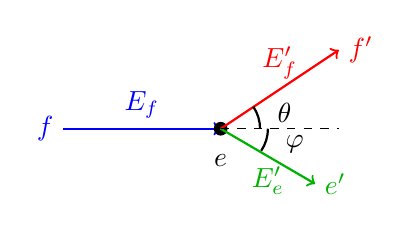
\begin{tikzpicture}
    \draw[->,thick,blue] (-2,0) -- (0,0) node[midway,above] {$E_f$};
    \draw[blue] (-2,0) node[left] {$f$};

    \draw[fill=black] (0,0) circle (0.08);
    \draw (0,-0.2) node[below] {$e$};

    \draw[->,thick,red] (0,0) -- (1.5,1) node[midway,above] {$E_f'$};
    \draw[red] (1.5,1) node[right] {$f'$};

    \draw[->,thick,green!70!black] (0,0) -- (1.2,-0.7)
    node[midway,below] {$E_e'$};
    \draw[green!70!black] (1.2,-0.7) node[right] {$e'$};

    \draw[thick] (0.5,0) arc (0:34:0.5);
    \draw (0.6,0.2) node[right] {$\theta$};

    \draw[thick] (0.6,0) arc (0:-34:0.5);
    \draw (0.7,-0.2) node[right] {$\varphi$};

    \draw[dashed] (0,0) -- (1.5,0);
  \end{tikzpicture}
  \caption{Ilustracja zjawiska Comptona. Foton $f$ ma długość fali $\lambda$.}
\end{figure}

W zjawisku zachowanny jest pęd oraz energia, co wraz z równaniem Comptona:
$$
(\lambda' - \lambda) \frac{m_ec}{h} = 1 - \cos\theta
$$
Pozwala nam w istocie wyprowadzić wszystkie niewadome w zjawisku.

$$
p_f + p_e = p_f' + p_e' \Rightarrow
\begin{cases}
  \frac{h}{\lambda} = \frac{h}{\lambda'}\cos\theta + p_e'\cos\varphi \\
  0 = \frac{h}{\lambda'}\sin\theta + p_e'\sin\varphi
\end{cases}
$$

$$
E_f + E_e = E_f' + E_e' \Rightarrow \frac{hc}{\lambda} + m_ec^2 =
\frac{hc}{\lambda'} + E_e'
$$

\section{Stan cząstki}

Z powyższych sekcji wiemy, że cząstka w mechanice kwantowej nie ma stricte
określonej pozycji ani pędu. Wynika to z zasady niepewności Heisenberga.
W mechanice klasycznej cząstki opisujemy parą $(x, p)$, czym opisujemy w
mechanice kwantowej? Mamy funkcję falową $\psi(x)$, gdzie $P(x) = |\psi(x)|^2$
opisuje prawdopodobieństwo znalezienia cząstki w $x$.

Elektron w okolicy atomu $1$ jest opisany przez funkcję falową $\psi_1(x)$.
Prawdopodobieństwo tego, że elektron jest w miejscu $x$ obok atomu $1$ opisuje
analogicznie $P_1(x) = |\psi_1(x)|^2$. Teraz wyobraźmy sobie, że
dodajemy drugi atom $2$ i nie wiemy obok
którego jest elektron. Na podstawie pomiarów możem określić, czy pomiary
odpowiadają $P_1(x)$, czy $P_2(x) = |\psi_2(x)|^2$.

Co jeśli elektron może być między cząstkami, czyli nie zakładamy, że należy
do jednej cząstki? Wtedy mówimy, że elektron jest w stanie $\psi_{1 +
2}(x) = \psi_1(x) + \psi_2(x)$. $P_{1 + 2} = |\psi_{1 + 2}|^2$.

\subsection{Pomiar}

Do momentu pomiaru, elektron w naszym przykładzie \textbf{nie ma
pozycji}. Założenie, że
jest obok jednej cząstki jest jak założenie, że cząstka przeszła przez jeden
otwór w eksperymencie Younga. Prawdopodobieństwo w mechanice
klasycznej i kwantowej działają zupełnie inaczej. W mechanice klasycznej
cząstki mają określony zawczasu stan. Pomiar, wykonany w danym czasie uzyska
zawsze jeden wynik. Identyczny pomiar wykonany w mechanice kwantowej może
uzyskać różne odpowiedzi.

Można to sobie wyobrazić w następujący sposób. W mechanice
klasycznej, prawdopodobieństwo $P(x)$ jest ewaluowane a priori.
Mechanika klasyczna jest deterministyczna i znając $(x, p)$ nie muszę
nawet robić pomiarów. W mechanice kwantowej $P(x)$ jest ewaluowane w czasie
rzeczywistym. Mechanika kwantowa nie jest deterministyczna.

\subsection{Funkcja}

$P(x) = |\psi(x)|^2$ musi być całkowalna po całej powierzchni.
Prawdopodobieństwo musi być skończone w końcu. Są od tej zasady
wyjątki, szczególnie cząstki, których całka rośnie wraz z rozmiarem
wszechświata.

Dla cząstki z określonym pędem $p$:
$$
\psi_p(x) = A\exp[\frac{ipx}{\hbar}]
$$
$A$ to czynnik normalizujący, wychodzący z konieczności
$1 = \int_{-\infty}^{\infty} |\psi_x(x)|^x dx$. Dla nieskończonego
wszechświata nie ma to sensu, bo $1 = |A|^2 \cdot \infty$.
Zatem zakładamy skończony wszechświat o obwodzie $L$:
$$
\psi_p(x) = \frac{1}{\sqrt{L}}\exp[\frac{ipx}{\hbar}]
$$
Warunek kwantyzacji ogranicza $p$ do:
$$
p_n = \frac{nh}{L}
$$
$$
\psi(x) = \sum_{p} A(p) \psi_p(x)
$$

\section{Model Bohra}

W modelu atomu Bohra, elektron porusza się wokół jądra wokół jednej z
dyskretnych
orbit. To też oznacza, że energia elektronu jest dyskretna lub zkwantowana.

\begin{figure}[H]
  \centering
  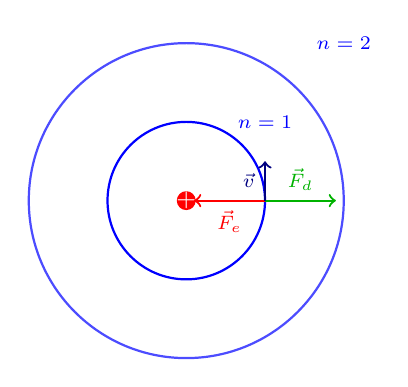
\begin{tikzpicture}
    \fill[red] (0,0) circle (0.12) node[white] {\small +};

    \draw[thick,blue] (0,0) circle (1);
    \draw[thick,blue,opacity=0.7] (0,0) circle (2);

    \node[blue] at (1,1) {\scriptsize $n=1$};
    \node[blue] at (2,2) {\scriptsize $n=2$};

    \draw[->,thick,green!70!black] (1,0) -- (1.9,0)
    node[midway,above] {\scriptsize $\vec{F}_d$};

    \draw[->,thick,red] (1,0) -- (0.1,0)
    node[midway,below] {\scriptsize $\vec{F}_e$};

    \draw[->,thick,blue!50!black] (1,0) -- (1,0.5)
    node[midway,left] {\scriptsize $\vec{v}$};

  \end{tikzpicture}
  \caption{Model Bohra atomu}
\end{figure}

Elektron na orbicie utrzymuje się w wyniku siły elektrostatycznej między
elektronem a jądrem.
$$
\frac{mv^2}{r} = k \frac{e^2}{r^2}
$$
$$
L = mvr = n\hbar
$$
Dla dowolnego ciała na orbicie:
$$
v = \frac{2\pi r}{T}
$$
gdzie $T$ jest czasem okresu orbity. Energie potencjalną można wyznaczyć z
pola elektrycznego.
$$
E_p = 2E_k = k\frac{e^2}{r}
$$
$$
E_k = \frac{1}{2}mv^2
$$

\subsection{Nieskończenie głęboka studnia potencjału}

Istnieje studnia potencjału. W zakresie $x \in (0, L)$ cząstka może się poruszać
swobodnie, potencjał jest zerowy. Poza tym obszarem potencjał jest
nieskończenie duży. długość studni ($L$) musi być równa całkowitej
wielokrotności połowy długości fali:
$$
L = n\frac{\lambda}{2}
$$
Trzeba też wykorzystać własności fali de Broglie
($\lambda=\frac{h}{p}$) aby uzyskać:
$$
p_n = \frac{nh}{2L}
$$

Postulat Bohra:
$$
\oint pdq = nh
$$

\subsection{Ciało doskonale czarne}

Ciało doskonale czarne, to koncept fizyczny, w którym rozważamy zachowanie się
energii, temperatury i promieniowana w doskonale czarnej wnęce. Założenie jest
takie, że ciało ma nie dopuścić do powrotnej emisji promieniowania.

W ciele doskonale czarnym zakłada się, że liczba modów oscylacyjnych jest dana
wzorem:
$$
N(\nu)d\nu = \frac{8\pi\nu^2}{c^3}d\nu
$$
Wynika to z $\nu = \frac{c}{\lambda}$ oraz $\lambda = \frac{2\pi}{k}$.
Gęstość energii na jednostkę częsości wyraża się:
$$
u(\nu, T) = N(\nu)\langle E \rangle
$$

\subsubsection{Katastrofa w ultrafiolecie}

W klasycznej teorii z zasady ekwipartycji energii wynika, że średnia
energia przypadająca na jeden stopień swobody układu oscylacyjnego jest równa:
$$
\langle E \rangle = k_BT
$$
Podstawienie $\langle E \rangle = k_BT$ do $u(\nu, T)$ daje nam wzór
Rayleigha-Jeansa na gęstość energii na jednostkę częstośći. Ten wzór jest
o tyle słaby, że całka po całym zakresie $\nu$ daje nam nieskończoną energię,
co jest nonsensem. Ten fenomen został nazwany katastrofą w ultrafiolecie.

\subsubsection{Wzór Plancka}

Planck rozwiązał problem z wzorem Rayleigha-Jeansa, wprowadzając inną
definicję $\langle E \rangle$. Podstawowym założeniem Plancka jest, że energia
pojedynczego oscylatora jest zkwantowana.
$$
E_n = nh\nu
$$
$$
\langle E \rangle = \frac{h\nu}{e^{\frac{h\nu}{k_BT}} - 1}
$$

\section{Obserwacje}

Pomiar $L$, wyrażony macierzą, może przyjąć wartości zgodne z jego wartościami
własnymi. Z reguły, poprzez $\ket{L = \lambda}$ zapisuje się wektor własny
stanu (macierzy) $L$, odpowiadający wartości własnej $\lambda$.

Wartość oczekiwana operatora $O$ w stanie $\ket{L = \lambda}$ jest równa:
$$
\langle O \rangle = \bra{L = \lambda} O \ket{L = \lambda}
$$
ta zależność jest prawdziwa, nawet dla transformacji, np.: $O = O'^2$.

Jeśli założymy, że $\Delta O$, jest określona przez odchylenie
standardowe ($\sigma$), to:
$$
\Delta O = \sqrt{\langle O^2 \rangle - \langle O \rangle^2}
$$

Prawdopodobieństwo wystapienia stanu (wektora) własnego $\ket{O = \psi}$
operatora $O$ w stanie $\ket{L = \lambda}$, jest dane wzorem:
$$
P(\ket{O = \psi}) = |\braket{O = \psi}{L = \lambda}|^2
$$

W stanie $\ket{\psi}$ w bazie $L$, zmierzyliśmy $L'$ i uzyskaliśmy wartość
$\lambda$. Dla takiego pomiaru możemy określić podprzestrzeń $L$, odpowiadający
stanom, które mogły doprowadzić do wyniku. Taką podprzestrzeń określamy:
$$
\Pi = \sum_{\lambda_i : \lambda_i^2 = \lambda} \ket{L =
\lambda_i}\bra{L = \lambda_i}
$$
Projekcja $\ket{\psi}$ na $\Pi$ daje nam stan po pomiarze $\ket{\psi'}$.
$$
\ket{\psi'} = \Pi \ket{\psi}
$$
$$
P(L' = \lambda) = \bra{\psi} \ket{\psi'}
$$

\section{Równanie Schrödingera}

$$
i\hbar \frac{\partial}{\partial t} \ket{\psi} = H \ket{\psi}
$$
gdzie $H$ to hamiltonian układu (dający energię układu), a $\psi(t)$ to stan
w czasie.

\end{document}
